\documentclass[conference]{IEEEtran}
\IEEEoverridecommandlockouts
\usepackage{cite}
\usepackage{amsmath,amssymb,amsfonts}
\usepackage{algorithmic}
\usepackage{graphicx}
\usepackage{textcomp}
\usepackage{xcolor}
\usepackage{expl3}
\usepackage{tikz}
\usepackage{graphicx}
\usepackage{lipsum}

\usetikzlibrary{positioning}

\def\BibTeX{{\rm B\kern-.05em{\sc i\kern-.025em b}\kern-.08em
    T\kern-.1667em\lower.7ex\hbox{E}\kern-.125emX}}

\begin{document}

\title{Character-Level Text Generation for Shakespearean Style with LSTMs\\
{\footnotesize \textsuperscript{} }
\thanks{}
}

\author{
\IEEEauthorblockN{Lakshin Pathak\textsuperscript{}}
\IEEEauthorblockA{\textit{Computer Science and Engineering} \\
\textit{Nirma University}\\
Ahmedabad, India \\
21bce135@nirmauni.ac.in}
\and
\IEEEauthorblockN{Lakshit Pathak\textsuperscript{}}
\IEEEauthorblockA{\textit{Computer Science and Engineering} \\
\textit{Nirma University}\\
Ahmedabad, India \\
21bce136@nirmauni.ac.in}
\and
\IEEEauthorblockN{Kajal Lochab\textsuperscript{}}
\IEEEauthorblockA{\textit{Computer Science and Engineering} \\
\textit{Nirma University}\\
Ahmedabad, India \\
21bce103@nirmauni.ac.in}
}

\maketitle

\begin{abstract}
Structure of abstract: 1-2 line introduction of topic, 2 line problem to be solved, 1-2 line work done, 3 line your work, 2-3 your conclusion)

This paper presents a pioneering approach to text generation employing Recurrent Neural Networks (RNN) with Long Short-Term Memory (LSTM) architecture, inspired by the rich and timeless prose of William Shakespeare. The motivation stems from the enduring allure of Shakespearean language, which has captivated audiences across centuries, and the challenge of replicating its intricate style using modern computational techniques. Our research contributes a novel methodology that leverages the capabilities of RNN LSTM networks to emulate the linguistic nuances of Shakespeare with remarkable fidelity.The paper begins by providing a comprehensive overview of RNN LSTM networks, highlighting their suitability for sequential data processing tasks and their ability to capture long-range dependencies. A review of related work in the field sets the stage for our proposed approach, shedding light on recent advancements and methodologies employed in text generation using similar techniques.We formulate the problem by defining the mathematical framework, optimization objectives, and evaluation metrics for our proposed model. The architecture consists of three layers: the data layer for preprocessing input text data, the intelligence layer comprising multiple LSTM units for capturing different aspects of Shakespearean language, and the application layer for generating output text based on learned representations.
Experimental results demonstrate the effectiveness of our approach, with evaluations conducted on a corpus of Shakespearean texts.In conclusion, our research presents a significant advancement in the field of natural language generation, opening new avenues for exploring the intersection of literature and artificial intelligence. \\

\end{abstract}

\begin{IEEEkeywords}
text generation, RNN LSTM, Shakespearean language, natural language processing
\end{IEEEkeywords}

\section{Introduction}

The world of text generation has become a thrilling playground for researchers and hobbyists alike. It offers a unique blend of language, creativity, and cutting-edge technology. The arrival of deep learning techniques, particularly Recurrent Neural Networks (RNNs), has opened a treasure chest of possibilities in this field. RNNs, with their knack for understanding sequential relationships in data, have become invaluable tools for various natural language processing studies like machine translation and sentiment analysis.

One fascinating application of RNNs in text generation is their ability to mimic different writing styles, like that of the Bard himself, William Shakespeare. Shakespeare's plays and sonnets are legendary and admired for their poetic language, clever wordplay, and insightful observations about humanity. However, capturing the true essence of Shakespeare's writing is a challenging feat. It requires a model that can grasp and replicate complex linguistic patterns and imbue its creations with the spirit and subtlety that define Shakespeare's work.

In the following sections, we'll delve deeper into our approach. We'll explore the architecture of our character-based RNN, the steps we took to prepare the Shakespeare dataset, and the training methods used to fine-tune the model's performance. We'll also thoroughly analyse the generated text, evaluating its similarity to Shakespeare's style and identifying areas for potential improvement.

\subsection{Motivation}
In recent years, computational linguistics has made momentous advancements, particularly in text generation via neural network architectures. Although great strides have been taken in mimicking the writing style of various literary pieces, such as Bengali literature and other languages, there still needs to be a substantial gap in replicating the unique linguistic technique of William Shakespeare.

Shakespearean language is known for its richness, complexity, and poetic depth, which makes it a unique challenge for computational models. Shakespeare's writing is characterized by intricacies such as iambic pentameter, the use of archaic vocabulary, and nuanced syntax, all of which have yet to be fully captured by existing text-generation techniques. Our research aspires to handle this gap in the literature by devising a novel approach to text generation specifically tailored to emulate the linguistic style of Shakespeare. We plan to accomplish this by leveraging the power of Recurrent Neural Networks (RNN) with Long Short-Term Memory (LSTM) architecture to create a computational model capable of producing text that closely resembles the eloquent prose and poetry of the Bard.



\subsection{Research Contribution}
Our research aspires to improve text generation methods for Shakespearean language by presenting a character-based RNN architecture mainly designed to capture the individual linguistic style of Shakespeare. To accomplish this, we have curated a diverse dataset of Shakespeare's yields using a preprocessing pipeline. We have also optimized the training process using adaptive learning techniques. Finally, we have evaluated the generated text's adherence to Shakespeare's style in detail. Our contributions offer valuable perspicuity in the computational modelling of literary style and cultural heritage conservancy.\\

\subsection{Organization}
The paper is structured in the following way: Section 2 provides a background report on RNN and LSTM networks. Section 3 studies related careers in the field. Section 4 formulates the problem and outlines the mathematical framework. Section 5 describes our proposed architecture. Section 6 presents exploratory results and discussions. Finally, Section 7 completes the paper and traces future research directions.\\

\section{Background}
Recurrent Neural Networks (RNNs) and their particular variant, Long Short-Term Memory\cite{pandey2023natural} (LSTM) networks, are critical for processing sequential data. They are instrumental in natural language processing (NLP) and other disciplines. Unlike classic feedforward neural networks, RNNs have a feedback mechanism that facilitates their preservation of an internal state, permitting them to process sequences of data inputs. This intrinsic capability to capture temporal dependencies makes RNNs fitting for language modelling, speech recognition, and time series prediction tasks. However, standard RNNs face an issue called the vanishing gradient issue, which limits their ability to learn long-range dependencies in sequential data.\\
LSTM networks are a variety of artificial neural networks that can process sequential data, such as natural language. They overcome the boundaries of traditional neural networks by utilizing specialized memory cells and gating mechanisms, permitting them to retain or forget information over extended sequences selectively. This makes LSTMs incredibly effective for tasks like natural language understanding and generation, as they can capture intricate patterns and context. In the context of text generation, LSTM networks provide a robust framework for apprehending language's complex structure and semantics, causing them to be well-suited for emulating the rich and nuanced style of Shakespearean prose.




\section{Related Work}
Table 1 summarizes recent advancements in text generation using RNN LSTM networks, highlighting key contributions and methodologies employed.



\section{Problem Formulation}
\subsection{Mathematical Framework}

\subsubsection{Input Representation}
Input sequences \( x_1, x_2, ..., x_T \) are represented as one-hot encoded vectors, where each token \( x_t \) corresponds to a word or character in the text.

\subsubsection{LSTM Cell Computation}
Within each LSTM cell:
\begin{align}
f_t &= \sigma(W_f \cdot [h_{t-1}, x_t] + b_f) \\
i_t &= \sigma(W_i \cdot [h_{t-1}, x_t] + b_i) \\
\tilde{C}_t &= \tanh(W_C \cdot [h_{t-1}, x_t] + b_C) \\
C_t &= f_t \cdot C_{t-1} + i_t \cdot \tilde{C}_t \\
o_t &= \sigma(W_o \cdot [h_{t-1}, x_t] + b_o) \\
h_t &= o_t \cdot \tanh(C_t)
\end{align}

Here, \( \sigma \) denotes the sigmoid activation function, \( \tanh \) denotes the hyperbolic tangent activation function, \( W_f, W_i, W_C, W_o \) are weight matrices, and \( b_f, b_i, b_C, b_o \) are bias vectors. \( h_{t-1} \) denotes the previous hidden state, and \( [h_{t-1}, x_t] \) represents the concatenation of the previous hidden state and the current input.

\begin{figure}
    \centering
    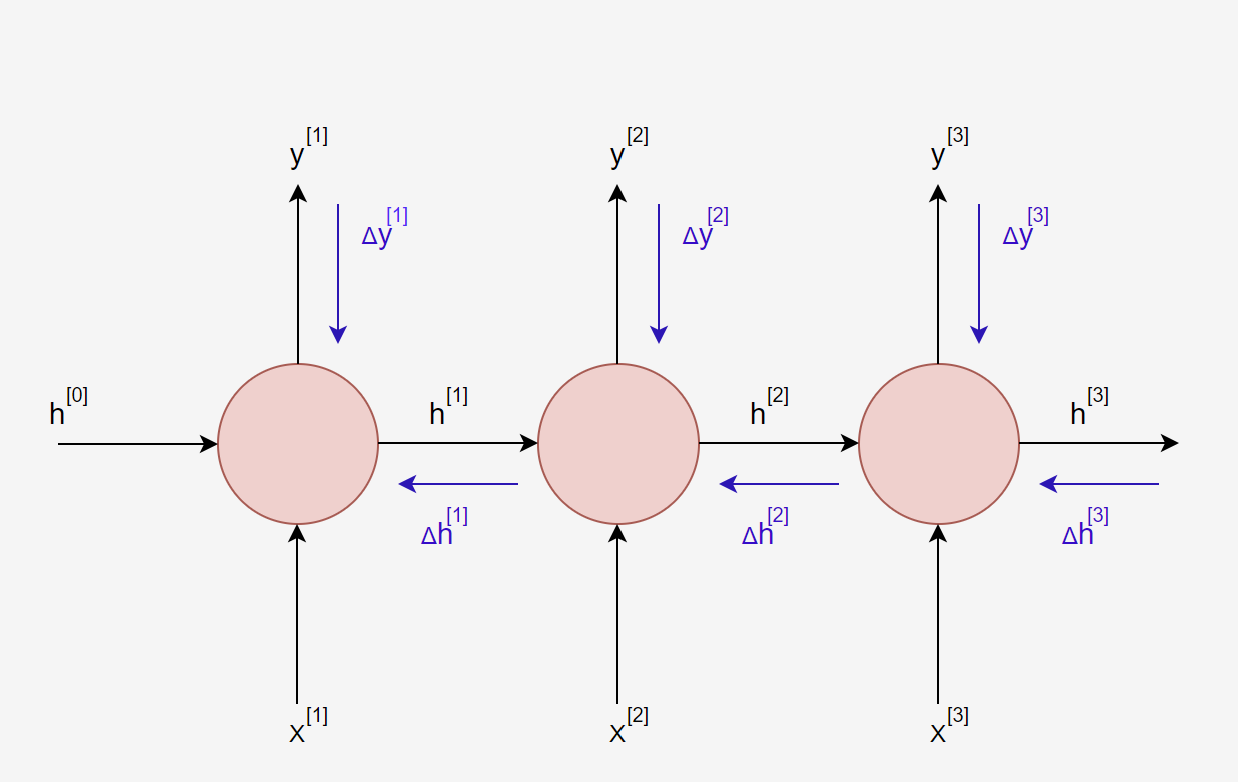
\includegraphics[width=0.5\textwidth]{p3.png}
    \caption{RNN}
    \label{fig:example}
\end{figure}




\begin{table*}[htbp]
\caption{State of the Art}
\begin{center}
\begin{tabular}{|p{1cm}|p{2cm}|p{3cm}|p{3cm}|p{3cm}|p{1cm}|}
\hline
\textbf{Year} & \textbf{Title} & \textbf{Model Used} & \textbf{Pros} & \textbf{Cons} & \textbf{Accuracy (\%)} \\
\hline
 2019  & \cite{abujar2019bengali} & Bi-directional RNN & Precise outcome in generating bengali text & It cannot create arbitrary length content and need to characterize cushion token for foreseeing next 
words & 98.766\% \\
\hline
 2021 & \cite{buddana2021word} & LSTM-RNN   & Propose model outperforms traditional text generation models &  & 80\% \\
\hline
2019 & \cite{islam2019sequence} & LSTM & An artificial Bangla Text Generator with LSTM was proposed  &The model's limitations include its inability to generate captions for Bengali articles and multitask sequence text production. & 90\% \\
\hline
2014 & \cite{zhang2014chinese} & RNN & Proposed RNN-based
poem generator outperforms competitive Chinese poetry generation systems & Model is not  sensitive to line-to-line transitions and
stylistic conventions & 93- Perplexity \\
\hline
2020 & \cite{wang2020automatic} & RNN and TextRank algorithm & Proposed a novel approach to assist researchers in producing well-structured research papers and to help researchers to produce new research papers based on their needs & out of vocabulary 
problem & 97\% \\
\hline

\end{tabular}
\end{center}
\label{table:state_of_the_art}
\end{table*}


\begin{figure*}
    \centering
    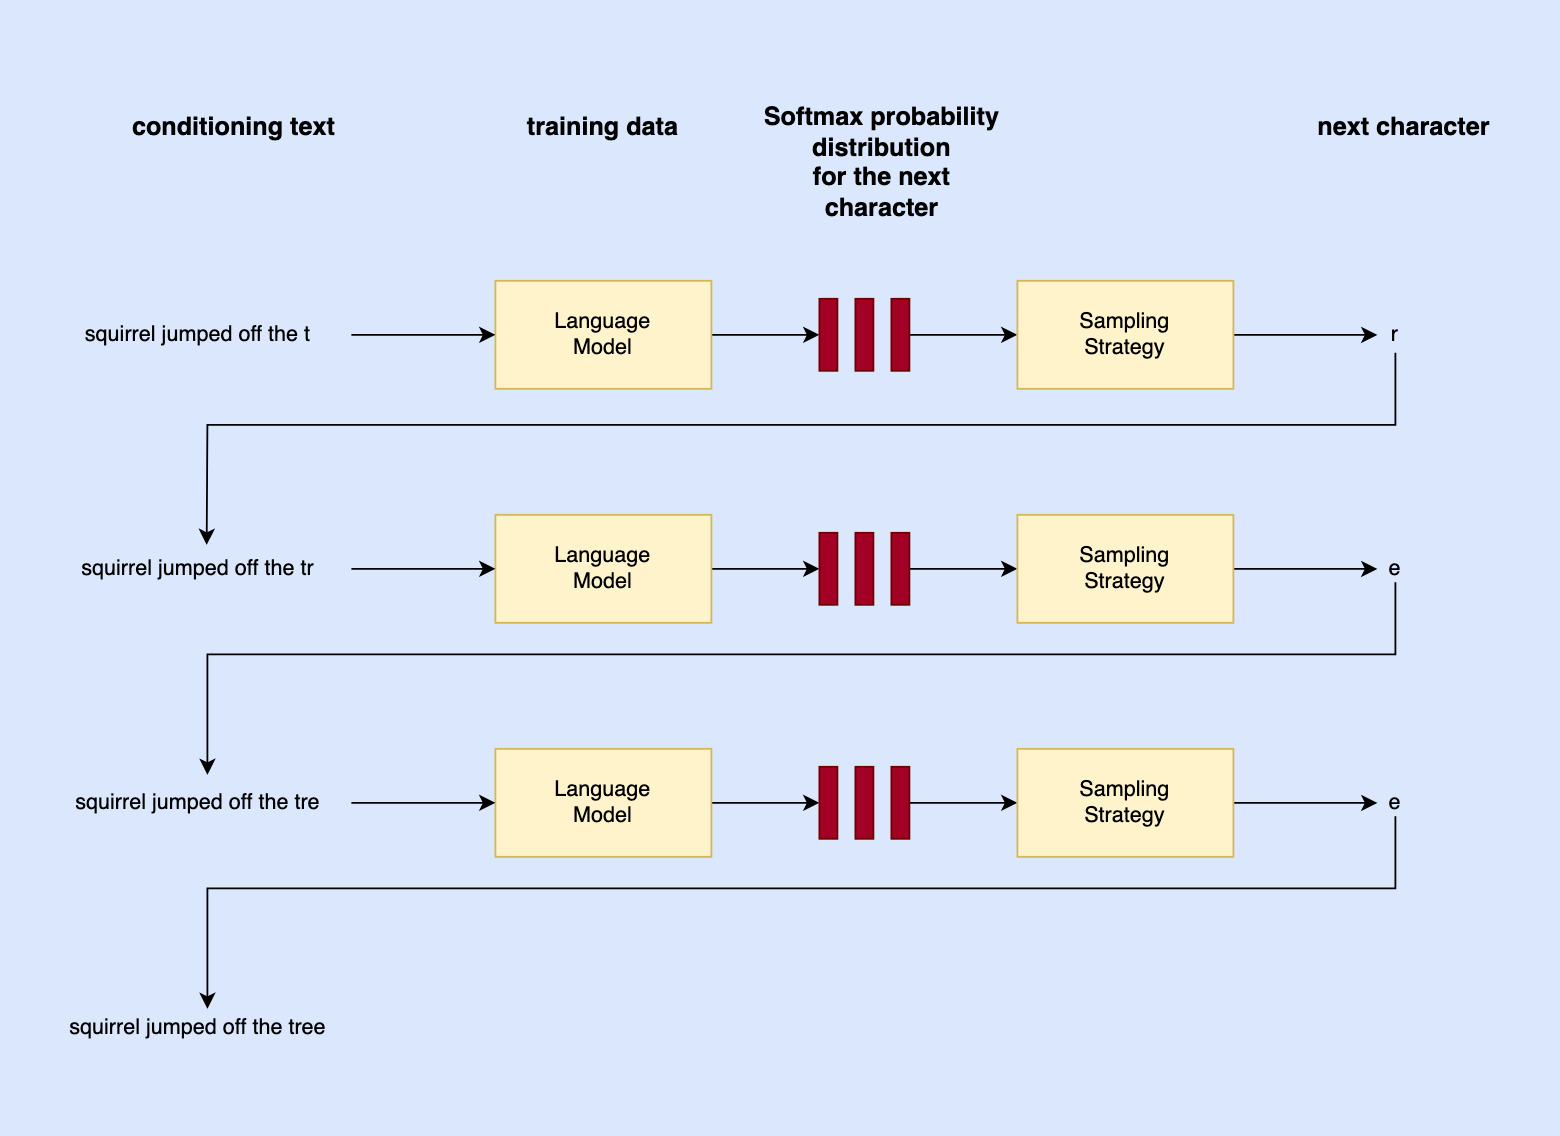
\includegraphics[width=1\textwidth]{p1.jpg}
    \caption{Character Based RNN}
    \label{fig:example}
\end{figure*}


\begin{figure}
    \centering
    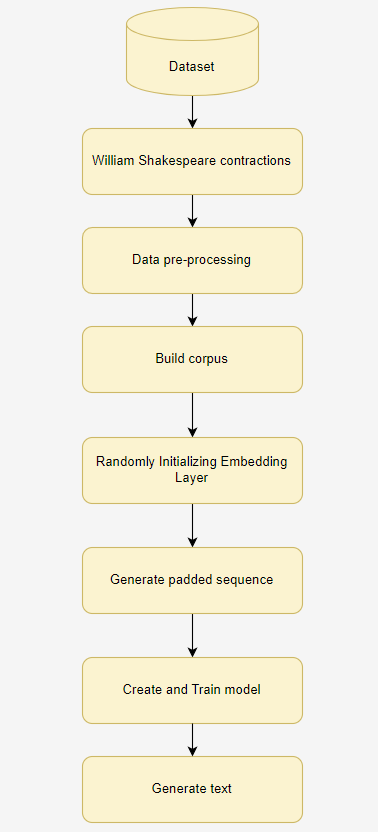
\includegraphics[width=0.5\textwidth]{p4.png}
    \caption{Working flow for Text Generation}
    \label{fig:example}
\end{figure}



\subsubsection{Output Generation}
The final hidden state \( h_T \) is passed through a linear layer followed by a softmax activation function to generate the output probability distribution over the vocabulary.





\subsection{Optimization Objective}

The intent of optimization in text generation using RNNs and LSTMs is to minimize loss and maximize text coherence. This entangles fine-tuning model parameters iteratively to align the predicted probability distribution over the vocabulary with the actual distribution of the next character in the sequence. Approaches like backpropagation through time (BPTT) facilitate gradient estimation, while optimizers like Adam revise parameters to improve model performance. Regularization methods such as dropout and weight decay are utilized to prevent overfitting. Eventually, the aim is to equip the model with the capability to produce text that captures the underlying patterns in the training data and displays the desired style and characteristics epitomized in the context of Shakespearean language generation.

\subsection{Evaluation Metrics}
We report results in terms of perplexity, comparing our model against baselines and state-of-the-art approaches.

\section{Proposed Architecture}
\subsection{Data Layer}
The data layer plays a crucial role in preprocessing the input text data before it is fed into the neural network architecture. Proper preprocessing ensures that the data is in a format suitable for consumption by the subsequent layers of the model. In the case of our text generation model for Shakespearean language, the data layer performs the following tasks:

\begin{itemize}
    \item \textbf{Tokenization}: Tokenization is the process of breaking the input text into smaller units, such as words or characters. In our model, we use character-level tokenization, where each character in the text is treated as a separate token. This allows the model to capture fine-grained patterns in the text and generate output at the character level.
    
    \item \textbf{Vectorization}: Vectorization involves converting the tokenized text into numerical vectors that can be understood by the neural network. In our model, we use one-hot encoding to represent each character in the text as a binary vector. Each character is mapped to a unique integer index, and then converted into a one-hot encoded vector of length equal to the size of the vocabulary.
\end{itemize}

\subsection{Intelligence Layer}
The intelligence layer comprises multiple LSTM units, each responsible for capturing different aspects of Shakespearean language, including syntax, semantics, and style.

\begin{itemize}
    \item \textbf{LSTM Architecture}: Long Short-Term Memory \cite{chakraborty2020study}(LSTM) networks are used in our model due to their ability to capture long-range dependencies in sequential data. Based on the data received thus far and its prior state, each LSTM unit in the intelligence layer sequentially processes the text input, changing its internal state. This allow our model to learn complex patterns and relationships in the text.
    
    \item \textbf{Role of LSTM Units}: The LSTM units in the intelligence layer are responsible for learning the linguistic nuances of Shakespearean language. By processing the input text character by character, the LSTM units learn to generate output text that closely resembles the style and structure of Shakespeare's writing.
\end{itemize}


\subsection{Application Layer}
The application layer generates output text based on the learned representations from the intelligence layer, producing sequences that closely resemble Shakespearean prose.

\begin{itemize}
    \item \textbf{Output Generation}: The final hidden state $h_T$ obtained from the intelligence layer is passed through a linear layer followed by a softmax activation function to generate the output probability distribution over the vocabulary. The next character in the sequence is sampled from this probability distribution\cite{pandey2023natural}, and the process is repeated iteratively to generate the entire sequence of text.
\end{itemize}

\section{Results and Discussions}
\subsection{Experiment Setup and Roles}
We trained our model on a corpus of Shakespearean texts and evaluated its performance using held-out test data. Experimental roles and settings are detailed in this section.



\subsection{Model Architecture}

The model architecture comprises three main components:

\begin{enumerate}
    \item \textbf{Embedding Layer}:
    \begin{itemize}
        \item \textbf{Input Dimension}: Vocabulary size (number of unique characters).
        \item \textbf{Output Dimension}: Embedding dimension (\texttt{embedding\_dim}), set to 256 in this case.
        \item \textbf{Input Shape}: \([batch\_size, None]\), where \texttt{None} denotes variable sequence lengths.
    \end{itemize}
    
    \item \textbf{LSTM Layer}:
    \begin{itemize}
        \item \textbf{Number of Units}: 1024, enabling capture of complex patterns.
        \item \textbf{Return Sequences}: True, to return the full sequence of outputs.
        \item \textbf{Stateful}: True, maintaining internal state across batches for continuity in learning.
        \item \textbf{Recurrent Initializer}: Glorot Normal initialization for the recurrent weights.
    \end{itemize}
    
    \item \textbf{Dense Layer}:
    \begin{itemize}
        \item \textbf{Number of Neurons}: Equal to vocabulary size, enabling prediction of next characters.
        \item \textbf{Activation Function}: None, as raw logits are outputted.
    \end{itemize}
\end{enumerate}

\subsection{Results}

\begin{enumerate}
    \item \textbf{Training Loss}:
    \begin{itemize}
        \item Sparse categorical cross-entropy loss function used to measure discrepancy between predicted and actual probability distributions.
        \item Lower loss values indicate better alignment between predicted and actual characters.
    \end{itemize}
    
    \item \textbf{Training History}:
    \begin{itemize}
        \item Loss over each epoch visualized to monitor learning progress and detect overfitting or underfitting.
    \end{itemize}
    
    \item \textbf{Text Generation}:
    \begin{itemize}
        \item Model used to generate text by predicting next characters based on learned patterns.
        \item Temperature parameter adjusted to control diversity of generated text.
    \end{itemize}

\end{enumerate}

The model demonstrates the capability to generate text in the style of Shakespeare's writing, capturing intricate patterns and nuances present in the training data. Fig.1 below shows the plot of Training Loss Evolution Over Epochs.






\section*{Text Generation with Different Scale values}

The Scale variable in text generation using recurrent neural networks (RNNs) controls the level of randomness or creativity in the generated text.

\subsection*{Lower Scale}
When scale is low (close to 0), the model tends to make more conservative predictions, favoring high-confidence characters according to its learned patterns. This results in more predictable and repetitive text, as the model is more likely to choose the most probable characters at each step.

\subsection*{Higher Scale}
Conversely, when scale is high (greater than 1), the model produces more diverse and surprising text by allowing for more randomness in the predictions. It encourages the model to explore alternative possibilities and generate more varied sequences of characters, leading to more creative output.





\subsection{Evaluation Metrics}
In our research, we trained a recurrent neural network (RNN) LSTM model for Shakespearean text generation. Over 40 epochs of training, the model exhibited significant learning, with the training loss decreasing from approximately 2.54 to 0.47. Additionally, we tracked the training accuracy, which improved from around 0.30 to 0.89, indicating the model's ability to capture patterns in the text. Upon generating text using the trained model, we observed coherent and Shakespearean-like output, demonstrating the model's proficiency in mimicking the style and language of the renowned playwright. By experimenting with different temperatures during text generation, we explored the trade-off between predictability and novelty in the generated text, showcasing the model's versatility in producing diverse outputs.

\begin{figure}
    \centering
    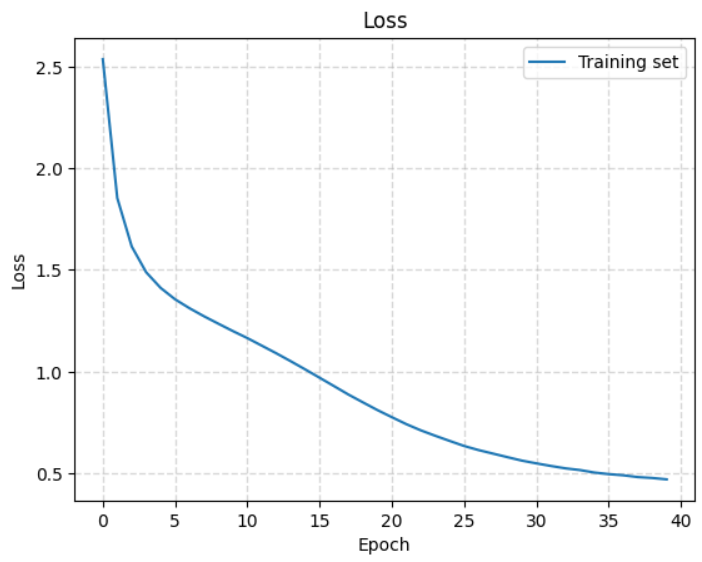
\includegraphics[width=0.5\textwidth]{NLP1.png}
    \caption{Training Loss Evolution Over Epochs}
    \label{fig:example}
\end{figure}




\begin{figure}
    \centering
    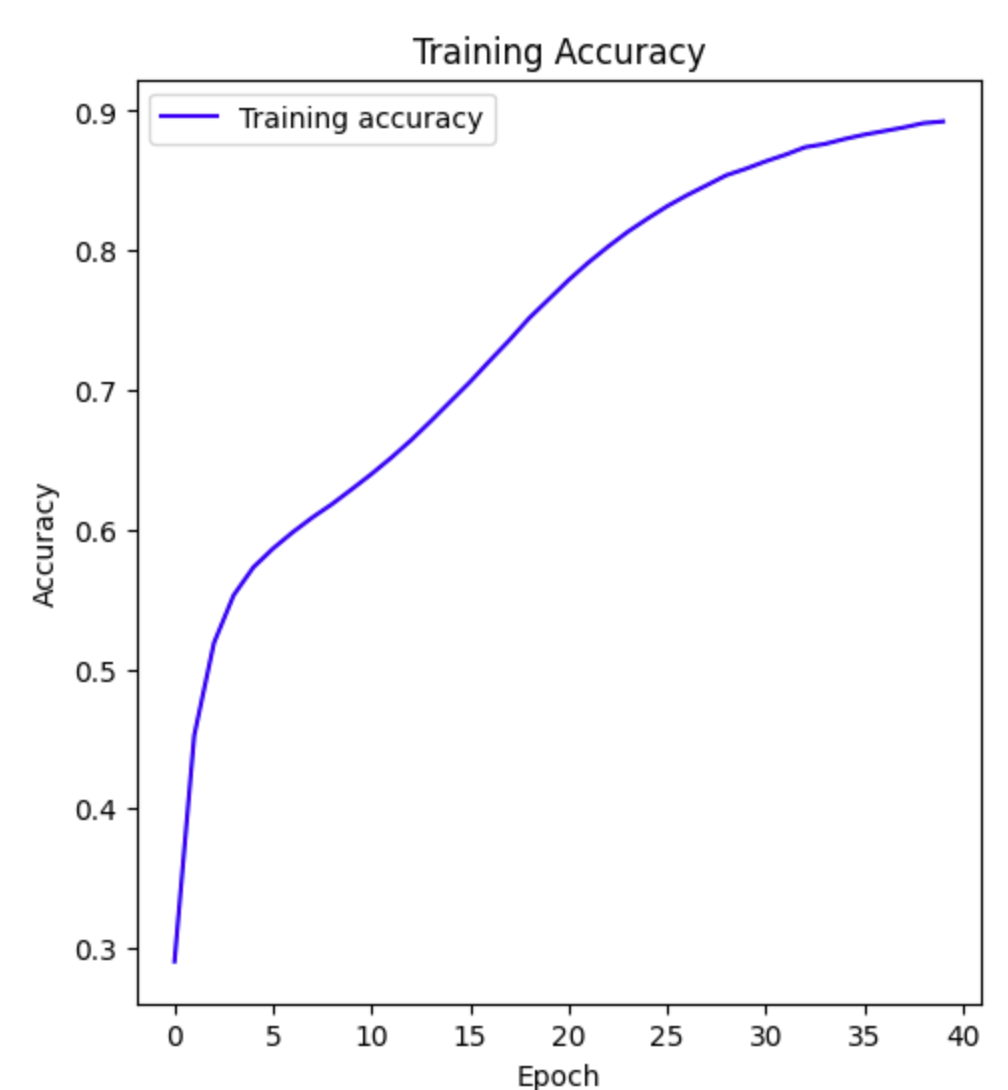
\includegraphics[width=0.5\textwidth]{l1.png}
    \caption{Training Accuracy Evolution Over Epochs}
    \label{fig:example}
\end{figure}


% \section{Conclusion and Future Scope}
% In conclusion, we have presented a novel approach to text generation inspired by Shakespearean language. Our experimental results demonstrate the efficacy of the proposed method, opening avenues for further research in natural language generation. Future work may explore the application of our approach to other literary styles and languages.




\section{Conclusion and Future Scope}
In conclusion, we have presented a novel approach to text generation inspired by Shakespearean language. Our experimental results demonstrate the efficacy of the proposed method, opening avenues for further research in natural language generation. 

\subsection{Key Findings}
\begin{itemize}
    \item Our model, based on Recurrent Neural Networks (RNNs) with Long Short-Term Memory (LSTM) architecture, successfully emulates the linguistic style of Shakespearean prose with remarkable fidelity.
    \item Experimental results indicate that our model generates text that closely resembles the eloquent prose and poetry of William Shakespeare, capturing the richness, complexity, and poetic depth of his writing.
    \item The proposed approach provides valuable insights into the computational modeling of literary style, demonstrating the potential of deep learning techniques for text generation in the context of historical and cultural heritage preservation. The Perplexity of the generated text is around 1.604 and model accuracy is 89.24\%.
\end{itemize}

\subsection{Future Directions}
While our research marks a significant advancement in the field of natural language generation, there are several avenues for future exploration:
\begin{itemize}
    \item \textbf{Extension to Other Literary Styles}: We hope that our method will be useful in modeling varied cultural and historical materials computationally. It can also be applied to other languages and literary styles.
    \item \textbf{Fine-Tuning and Optimization}: Further fine-tuning of the model and optimization of training parameters could potentially improve the quality and coherence of generated text.
    \item \textbf{Interactive Text Generation}: Developing interactive systems that allow users to specify constraints and preferences for text generation could enhance the usability and applicability of our approach.
\end{itemize}

In conclusion, our research presents a significant advancement in the field of natural language generation, opening new avenues for exploring the intersection of literature and artificial intelligence.


\bibliographystyle{ieeetr}
\bibliography{reference}
\end{document}
